\section{Auswertung}
\label{sec:Auswertung}

\subsection{Vorbereitung}
Bei der Vorbereitung wurde beim linken Schwingkreis eine Eigenfrequenz von $f_{\text{eigen}}=30.61 \si{\kilo\hertz}$ bei einer
Phasendifferenz von $\SI{0}{\degree}$ gemessen. 
Der verstellbare Kondensator wird so eingestellt, dass der rechte Schwingkreis die gleiche Eigenfrequenz hat, wie der linke.
Die Referenzwerte der Bauteile sind $C=\SI{0.8015}{\nano\farad}$ und $L=\SI{32.351}{\milli\henry}$.
Die Anzahl der Maxima, beziehungsweise Minima, sind in \autoref{tab:schwing_maxima} aufgeführt. Außerdem ist die 
Dauer einer Schwebung aufgetragen.


\begin{table}
  \centering
  \caption{Anzahl Maxima der Schwebung.}
  \label{tab:schwing_maxima}
  \begin{tabular}{c c c}
      \toprule
      {$C_K \:/\: \si{\nano\farad}$} & Schwingungsmaxima & $\Delta t\:/\: \si{\micro\second}$ \\
      \midrule
      9.99  & 13 & 235 \\ 
      8.00  & 11 & 195 \\ 
      6.47  & 10 & 155 \\ 
      5.02 & 8 & 125 \\ 
      4.00 & 7 & 100 \\
      3.00 & 6 & 75 \\
      2.03 & 4 & 50\\ 
      \bottomrule
  \end{tabular}
\end{table}

\subsection{Fundamentalschwingung}
Im folgenden werden die beiden Fundamentalschwingungen in Abhängigkeit der Kopplungskapazität $C_{\text{K}}$ des Kopplungskondensators
bestimmt. 


\begin{table}
  \centering
  \caption{Fundamentalschwingungen}
  \label{tab:aufgabeC}
  \begin{tabular}{c c c c c}
      \toprule
      {Maxima 1 $\;/ \si{\kilo\hertz}$} & {Maxima 2 $\;/ \si{\kilo\hertz}$} & {$V_1 \:/\: \si{\milli\volt}$} & {$V_2 \:/\: \si{\milli\volt}$} & {$C_K \:/\: \si{\nano\farad}$} \\
      \midrule
      38 & 49 & 60 & 110 & 9.99 \\
      40 & 50 & 55 & 110 & 8.00 \\
      40 & 50 & 55 & 110 & 6.47 \\
      38 & 55 & 50 & 110 & 5.02 \\
      40 & 58 & 50 & 105 & 4.00 \\
      40 & 62 & 50 & 105 & 3.00 \\
      40 & 73 & 50 & 100 & 2.03 \\
      40 & 76 & 55 & 95 & 1.01 \\
      \bottomrule
  \end{tabular}
\end{table}


\begin{figure}
  \centering
  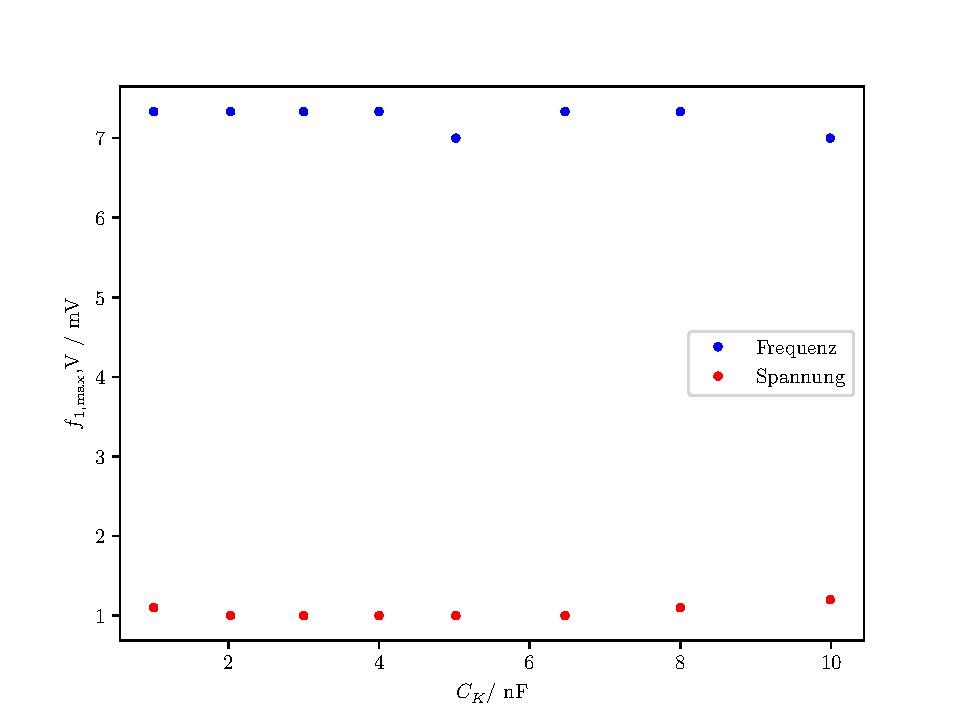
\includegraphics{freq1.pdf}
  \caption{Die aufgenommenen Messwerte}
  \label{fig:freq1}
\end{figure}

\begin{figure}
  \centering
  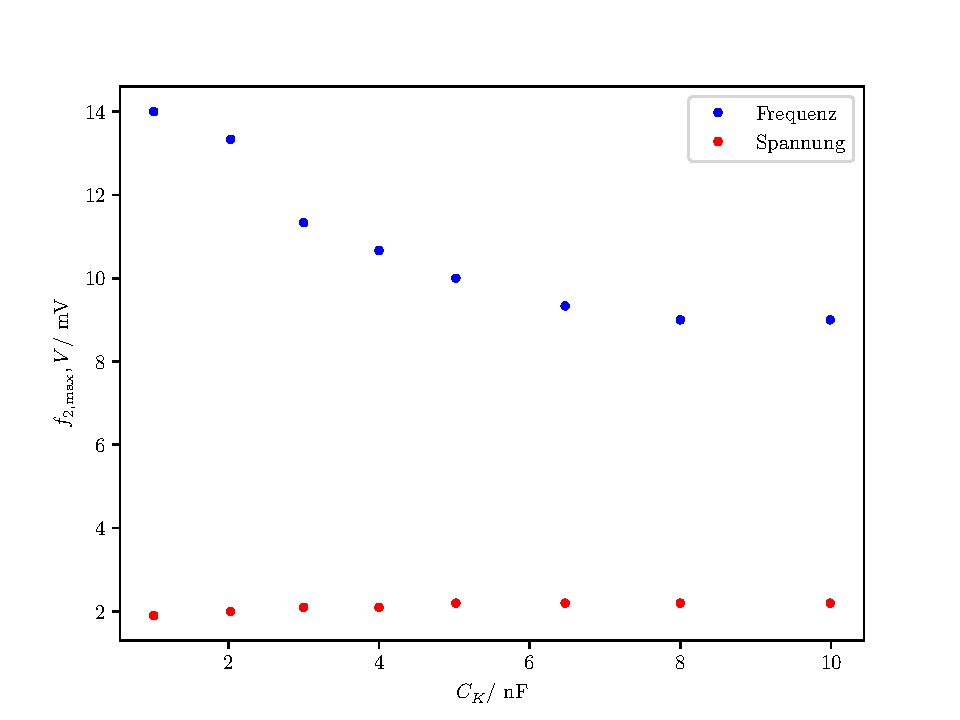
\includegraphics{freq2.pdf}
  \caption{Die aufgenommenen Messwerte}
  \label{fig:freq2}
\end{figure}





%Siehe \autoref{fig:plot}! Ich weiß nicht, was das hier überhaupt sein soll. Das mach ein Siehe Abbildung ! in das Protokoll.
% Aber wofür ist das gut?
